\section{РАЗРЯДНЫЙ КОНТУР}

Дан разрядный контур, который видно на рисунке \ref{img:con}.

\begin{figure}[H]
    \centering
    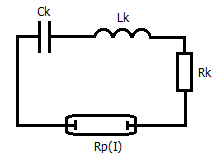
\includegraphics[scale=1]{img/scheme.png}
    \caption{Разрядный контур}
    \label{img:con}
\end{figure}

\section{СИСТЕМА ОДУ}

Получена система дифференциальных уранений (формула \ref{eq:diff}).

\begin{equation}\label{eq:diff}
    \begin{cases}
        L_\text{к}\frac{dI}{dt} + (R_\text{к} + R_p) I - U_c = 0 \\
        C_\text{к} \frac{dU_c}{dt} = -I \\
    \end{cases}
\end{equation}

Необходимо решить систему и построить графики $I(t), U_c(t), I\cdot R_p(t), R_p(t), T_0(t)$.

Cопротивление газоразрядной трубки, находится в зависимости от силы тока:

\begin{equation}
    R_p(I) = \frac{l_{\text{э}}}{2 \pi R^2 \int_0^1 \sigma(T(z))zdz}
\end{equation}

Для нахождения $T_0, m \sigma$ даны таблицы, к которым применялась интерполяция.

Система уравнений решается методом Рунге-Кутта 4 порядка для системы ОДУ.

\begin{equation*}
    y_{n+1} = y_n + \frac{k_1 + 2k_2 + 2k_3 + k_4}{6},
\end{equation*}

\begin{equation*}
    z_{n+1} = z_n + \frac{q_1 + 2q_2 + 2q_3 + q_4}{6}
\end{equation*}

, где

\begin{equation*}
    k_1 = h_n f(y_n, z_n), ~~q_1 = h_n \varphi (y_n)
\end{equation*}

\begin{equation*}
    k_2 = h_n f (y_n + \frac{k_1}{2}, z_n + \frac{q_1}{2}),~~ q_2 = h_n \varphi(y_n + \frac{k_1}{2})
\end{equation*}

\begin{equation*}
    k_3 = h_n f (y_n + \frac{k_2}{2}, z_n + \frac{q_2}{2}), ~~q_3 = h_n \varphi(y_n + \frac{k_2}{2})
\end{equation*}

\begin{equation*}
    k_4 = h_n f (y_n + k_3, z_n + q_3, ~~q_4 = h_n \varphi(y_n + k_3)
\end{equation*}

\section{ЛИСТИНГИ}

\begin{lstlisting}[caption=Интерполяция]
double Interpolation::get(Point *table, double x, unsigned short int len)
{
    int index = -1;
    for (int i = 1; i < len; ++i) {
        if (x >= table[i - 1].x && x <= table[i].x) {
            index = i;
        }
    }

    if (index == -1) {
        if (x <= table[0].x) return table[0].y;
        else return table[len - 1].y;
    }

    double x0 = table[index - 1].x;
    double y0 = table[index - 1].y;
    double x1 = table[index].x;
    double y1 = table[index].y;
    return y0 + ((y1 - y0) / (x1 - x0)) * (x - x0);
}
\end{lstlisting}

\begin{lstlisting}[caption=Интегрирование методом парабол (Метод Симпсона)]
double Mathematics::integral(double z, double I)
{
    return Interpolation::getSig(T(z, I)) * z;
}

double Mathematics::simpson(double a, double b, double I)
{
    double h = (b - a) / _n;
    double k1 = 0, k2 = 0;

    for (int i = 1; i < _n; i += 2) {
        k1 += integral(a + i * h, I);
        k2 += integral(a + (i + 1) * h, I);
    }

    return h / 3.0 * (integral(a, I) + 4 * k1 + 2 * k2);
}
\end{lstlisting}

\begin{lstlisting}[caption=Решение системы уравнений методом Рунге-Кутта]
void Mathematics::iteration()
{
    double k1 = f(_I, _Uc);
    double m1 = g(_I);

    double k2 = f(_I + _tau * (k1 / 2.0), _Uc + _tau * (m1 / 2.0));
    double m2 = g(_I + _tau * (k1 / 2.0));

    double k3 = f(_I + _tau * (k2 / 2.0), _Uc + _tau * (m2 / 2.0));
    double m3 = g(_I + _tau * (k2 / 2.0));

    double k4 = f(_I + _tau * k3, _Uc + _tau * m3);
    double m4 = g(_I + _tau * k3);

    _I  += _tau * ((k1 + 2 * k2 + 2 * k3 + k4) / 6.0);
    _Uc += _tau * ((m1 + 2 * m2 + 2 * m3 + m4) / 6.0);
}
\end{lstlisting}

\end{document}
